\documentclass[letterpaper, 10 pt, conference]{ieeeconf}

\IEEEoverridecommandlockouts
\overrideIEEEmargins

\usepackage{times}
\usepackage{mathptmx}
\usepackage{amsmath}
\usepackage{amsfonts}
\usepackage{amssymb}
\usepackage{graphicx}
\usepackage{multicol}
\usepackage[utf8]{inputenc}
\usepackage{array}
\usepackage{lipsum}
\graphicspath{{images/}}
\usepackage{parskip}
\usepackage{indentfirst}
\usepackage{courier}
\usepackage{wrapfig}
\usepackage{caption}
\usepackage[left=1.5in, right=1in, top = 1in, bottom = 1in]{geometry}
\usepackage{float}
\usepackage[ruled]{algorithm}
\usepackage{algpseudocode}
\usepackage{graphicx}
\usepackage{url}
\usepackage{cite}
\usepackage{rotating}
\usepackage{subcaption}

\parindent 10pt
\parskip 2ex

\begin{document}

\begin{center}
	\huge Critical Encounters
	
	\large Hunter Figueroa, Zachary Painter, Jacob Spigle, \& David Akridge
	
	\large Department of Electrical Engineering and Computer Science, University of Central Florida, Orlando, Florida, 32816-2450
\end{center}

\

\begin{abstract}
	This paper presents, in detail, the design process for creating our website, Critical Encounters. Critical Encounters is a web-based platform designed to streamline the process
	for players of the d20 Game System to create, test, and play through their own
	creations, including encounters and monsters, in order to play more effectively
	in a live setting. Users are able to publicly post their created encounters for
	others to play through and review, and utilize our stress-tester for more in-depth
	statistics about their creation.
\end{abstract}

\small \textbf{\textit{Index Terms}--- Creativity, crowdsourcing, digital simulation, internet, user centered design.}

\

\section{Introduction}

Role-playing games are games where players act as their characters. Usually
in person, around a table, and controlled by the players speaking their actions
in turn. This might not always be done by speaking in-character, but rather by
following this basic structure:
\begin{enumerate}
	\item The GM describes the environment.
	\item The players describe what they want to do.
	\item The GM narrates the results of the characters actions.
\end{enumerate}
\par
There are countless possible character, monster, and scenario possibilities when
constructing a tabletop role-playing campaign, however, it is hard and sometimes
impossible to sift through them all and find the perfect encounter. Not only that,
but once you commit to a game or role-playing decision you are forced to see it
through to completion in order to retain the game’s continuity. Players get one
chance to design their character at the very start of a session, and once they do,
that character’s path cannot be meaningfully changed. Spending so much time
working on a character, and then coming to the first session to find out that they
are severely unprepared for the tasks they are presented can be harrowing. On the
other side, the GM spends so much time outside of the game to prepare a story
and encounters that challenge the Players, so when that GM accidentally wipes
out the entire team of Player Characters (PCs) in one unbalanced encounter, or
if the PCs simply walk through a fight that was meant to challenge them for the
remainder of the session, the GM feels they have failed the PCs in presenting a
good game. \par
This project presents a service that can be used by both GMs and players to
test out their characters, encounters, team builds, or boss fights in a simulated
environment. This allows users to figure out just how well their creation holds
up to the requirements that they have set for themselves, and perfect them to
ensure the most enjoyable experience in a live game encounter.
This project seeks to develop a service that allows a user to create an encounter
that follows the rules of the d20 Game System. The creator streamlines the refining
process by easily being able to simulate the encounter. By allowing the player or
GM to import their character’s/monsters’ statistics and equipment, they then
can play against an automated opponent or opponents using that creation. Encounters have the ability to be rapidly simulated over and over to display
statistics about the encounter the help improve the encounter. To further enhance
a user’s ability to test and refine encounters and PCs, users are able to upload
and share their encounters to their public space where others can try their own
creations’ skills in that creator’s setting.

\section{Overview of Requirements}

This project was pitched by the group in the beginning of the Senior Design I semester, and as such, did not have a formal sponsor throughout the development process. The scale of the project and thus the requirements that the website Critical Encounters would achieve was based on the aspects that we felt were important to have completed by the end of the Senior Design II term. We knew that by the end of the formal project deadline we would have the following completed:
\begin{enumerate}
	\item Website hosted where it could be accessible from any device.
	\item Encounter Creator Tools present so users could invent their own combat centric encounters inside Critical Encounters, and the ability to host them on the website in their own space, their ``Arena''.
	\item Combatant Creation, where users could customize their own PC or monster.
	\item Battlefield where users could simulate a full encounter using either their own created encounter or those hosted by other users on the website against a DM or PC A.I. simulation, while using their own created PC or monster against the encounter creator's combatants present in the encounter.
	\item After completing an encounter on the website, users would be able to view statistics about the combat and review for their own usage. Users would also be encouraged to leave a review of the played encounter so the creator would receive feedback as well.
	\item The ability for users to save/load ongoing combat encounters.
	\item Users would be able to search for Arenas \& Encounters, while also being able to filter those results by tags, ratings, and time since the encounter was uploaded.
	\item An Encounter Diagnostic Tool would be implemented to allow users to run the system through a large amount of testing all at once, and receive statistics aggregated from those tests in order to better adjust their encounter for live gaming. 
\end{enumerate}

\section{High Level Block Diagram}
	\begin{figure}[H]
	\centering
	\centerline{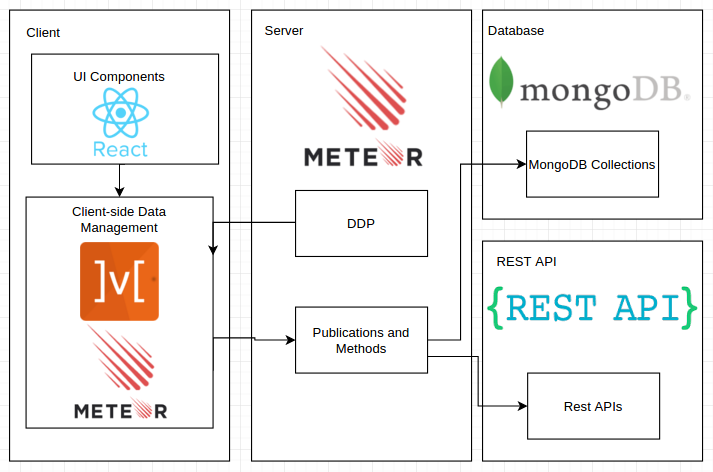
\includegraphics[scale=.3]{high_level_block_diagram}}
	\caption{High Level Block Diagram}
	\label{fig: High Level Block Diagram }
	\end{figure}

We have implemented a Client-Server Design structure that is commonly used
with web applications such as Critical Encounters. There are three areas of production
in this high-level design: Server, Database/Rest API and Client-Side. The UI
components are developed in REACT and control the the MVC system.
Data management on the client-side are managed by MobX and Meteor, the
latter of which serves as the point of contact with the server-side of the app.
The server is developed in Meteor, and is responsible for contacting
the database, developed in MongoDB and performing REST API commands when
necessary.
The relationship between client and server is a pseudo model-view-controller
architecture. Where REACT acts as the as application’s view and Meteor/-
MobX acts as both the controller and the model. Meteor with MobX automatically manages the data flow, client state, and client rendering. \par
Meteor uses an ORM/MERN, Object-relational mapping / MongoDB
- Express - React, stack design pattern. It focuses on model driven development,
in which the models are shared between the server and the client. This
is seen most clearly seen in the MiniMongo database cache that is accessible by
the font-end front end and can asynchronously update the MongoDB REST API
is implemented automatically which translates to automatic database updates.

\section{Hosting}
Using Google Domains, we procured www.critical-encounters.com, and by using this URL, users will be able to connect with our database to create their own encounters.
We are utilizing Amazon Web Services (AWS) for hosting Critical Encounters on the Internet.  Specifically, we are using the Amazon Elastic Compute Cloud (Amazon EC2), which is a web service that provides resizable computing capacity. The Amazon EC2 instance also allows us to connect to the server via the AWS Command Line Interface (CLI). We have connected to this service by going through Secure Shell (SSH) in order to set up our configuration on the server. Currently the instance we have chosen is a General Purpose t2.micro instance, and it is a Linux Server running Ubuntu OS 16.04. Amazon essentially leases these servers out to its' clients, and because it is scalable, we are able to increase the amount of servers available to us at any one time, or decrease the instances if necessary. This is perfect for running optimally at high-traffic times of day, and we will be taking advantage of this feature in the ongoing development and continual support of Critical Encounters. To bring our Meteor project from our local development computers and onto the AWS instance, we utilized a tool called ``mup'', which makes hosting with Meteor to AWS incredibly simple. We can configure our MongoDB and Meteor project using local configuration files and settings, and through a few simple commands mup will build a local version of the project, grab a snapshot of the database (actually using the fixtures.js file to create it the first time), and host the website on the Linux Server's IP. It is important to note that during initial testing and after development changes to Critical Encounters (specifically on the MongoDB side), it is necessary to SSH into the AWS instance and bring in the new schema available to keep the website functional with the new code changes.
\section{D20 Game System}
Critical Encounters' logic and customization is built around the d20 Game System, an open-license set of rules and statistics that can be used for creating tabletop games or in our case, applications that assist users using this system. There are many popular games that use this system, the most famous being Dungeons \& Dragons, Pathfinder, and more recently: Starfinder. \par
The d20 game system has variations from game to game whether it be changes
to name, function, or practicality. Despite this, generally many the main qualities
that the game styles have don’t tend to stray too far from one another. While on
this project, it is crucial that Critical Encounters should provide a broad enough
experience to appease the largest portion of d20 games as possible so that players
can apply their encounters to whatever d20 system they’d like. \par
More information about the d20 game system is available in \cite{c4}.

\section{Major Components}
A website is a multifaceted system created through many different aspects of web development. These aspects include web design, web publishing, web programming, and database management. Development of a web application utilizes these same aspects. Here we will cover the UI, Application Design, A.I..
\subsection{UI}
The approach we took to user interface (UI) design was focused on a simplistic
and familiar look and feel to allow for easy accessibility to new users while the
website itself still retaining focus on the encounter tester. The template the website
utilizes is reminiscent of the design that many social media sites take. Take for
instance sites like Twitter, Facebook, and YouTube.
\subsubsection{NavBar}
The site also uses the the single-page application structure that allows for easy
traversal. The persistent navigation bar has Critical Encounters’
name and logo in the top left of each page which redirects users back to the homepage,
a search bar in the top of each page which redirects users to the Encounter
Browser page, and the user’s username in the top right of each page that links to
the user’s Arena.
\subsubsection{Login/Registration}
The registration page for Critical Encounters requires the user’s
desired username, their email address, and their password. Users are directed to
the registration page from the Dashboard or from clicking the “Register” link on
the login page. The login page for Critical Encounters prompts users for their
credentials to log in. Beneath the username/email address \& password fields is a
“Register” link to the registration page and a “Forgot Password?” to a password
retrieval service. Users are directed to the login page by clicking the “Login” link
on the navbar, or after attempting to access content that requires an account. (i.e.
accessing the Battlefield, Arena, subscribing, reviewing, etc.)
\subsubsection{Dashboard}
The Critical Encounters’ Dashboard features notable encounters,
updates, and community events in the highlight wheel at the forefront of the page.
Below the highlight wheel is a list of recommended encounters that either we the
developers suggest to the community, or recommended list that is influenced by
the user’s recent search history.
The Dashboard doubles as a homepage for the Critical Encounters website.
\subsubsection{Encounter Browser}
The Critical Encounters’ Encounter Browser acts as a search results
page for queries entered in the search bar. From this page a list of filtered
encounters is presented to the user. The user may also filter those results further
by selecting settings from the dropdown menu revealed by the ’Filter’ button.
Through this process we can be sure to provide users with encounters that help
with creation or spark their own imagination.
\subsubsection{Arena}
Each Critical Encounters user is provided a page to host their published encounters
for the rest of the community to access, their Arena. From the Arena
page is where users are redirected to encounter creation within the
Battlefield by clicking the “Encounter” tab on the Arena page, then clicking the
‘+’ sign above their previously created encounters. Likewise, users can click on
the “Combatants” tab to display their created combatants as well as create new
combatants by clicking the ‘+’ sign on the page. Users also have the ability to edit
their Arena, listing their created encounters in whatever order they wish, whether
done manually or by analytics (Plays, Win Rate, Rating).
\subsubsection{Combatant Creation}
The Combatant Creation tab will expand when the ‘+’ is clicked on a
user’s Arena page to reveal all the parameters that are necessary to make a base
character. We have opted out of including sections for roleplay aspects at the
moment (Personality Traits, Ideals, Bonds, Flaws, etc.), and have instead focused
on the ability scores, class, level, background (for ability proficiency purposes),
race, and alignment. Actions, which include Weapons, Spells, and general combat
actions can be added to a character’s stat sheet using the tool by clicking ‘+’ next
to each. Feats can also be added to a character’s stat sheet in the same manner.
\subsubsection{Encounter Page}
Each encounter created in Critical Encounter is given an encounter page, from
which user’s navigate to in order to start playing the encounter. At the top of the
encounter page is the encounter’s name, followed by the username of its’ creator. The encounter page also includes a description of the encounter as well as statistics aggregated from playthroughs.
\subsubsection{Battlefield}
The Battlefield is where users will create, edit,
and play their encounters. Because of its importance we have put a lot of thought
into the requirements, design, and implementation plans. Both the front-end and
back-end work closely on this component because the battlefield is the stage
that our AI will be able to show its capabilities.
\begin{itemize}
	\item \textit{Board:} The board is where all the environment, obstacles, and combatants are rendered.
	The board is a 2D top down arena, inspired by popular strategy games
	such as Civilization. The board is composed of checkerboard likes faces Each of
	which represent 5 feet of space in the game world. Obstacles and combatants will
	be rendered inside of these spaces. Obstacles and combatants can be hovered over,
	selected, as well as be clicked and dragged into other spaces within the combatants
	movement range. If one of the combatants or obstacles are clicked their details
	and descriptions will appear in the sidebar. \\
	\item \textit{Sidebar:} In the sidebar the user can view a combated or obstacles description and statistics.
	\begin{itemize}
		 \item \textit{Game Mode:} After an encounter starts there will be a number above each combatant to represent the number that they rolled for their initiative (this decides the order in which actions take place during a combat encounter). There is also a green bar in place to represent each combatants' current health. During a combatants' turn, upon clicking their tile in the sidebar (or by clicking on their image in the battlefield map) the tile will expand to show all the the combatants available actions, and the `price' associated with that action. From there the user may select the action they would like to perform, and click the target in the battlefield map to perform the selected action. \\
		 \item \textit{Creation Mode:} The sidebar will also be used in the creation mode
		of the battlefield. In the sidebar the user will be able to search, select, in drag
		combatants and obstacles onto the battlefield. They can also view and edit any
		of the stats using a form contained in the sidebar, under the Character Creation
		Tools menu. Here will also be where the user can make adjustments to combatant
		AI whether it’s setting its aggressiveness level or selecting one of our built in my
		presets. In other words the sidebar is where the user will manage all the details
		of the encounter in both creation and game mode. \\
	\end{itemize}
	\item \textit{Battle Log:} The Battle Log is where all of the messages attached to combat an
	encounter actions will be displayed. They will supply the user with an up-to-date
	text rendition of the encounter. It includes messages like, ”The Goblin struck
	the cleric with a sword dealing 5 points of slashing damage”, ”The wizard cast
	Firebolt at the ogre but it missed”, and ”The Rogue hides behind the barrel the
	dragon does not seem to notice him”. Notice how the battle log will include whimsical and sometimes graphic descriptions of the events that occur ``in-game'' due to the actions the user chooses to take when playing through an encounter. We believe this will keep Critical Encounters' battle log from becoming a large block of text that is a nuisance to read through. The log should be something interesting to read through, and help simulate conversation that occurs during a combat in a live tabletop gaming session.
\end{itemize}
\subsection{Application Design}
This section describes the Critical Encounters web applications' server, database, \& client side design.
\subsubsection{Server Design}
Critical Encounters uses Meteor, a full-stack JavaScript platform for developing modern web and mobile
applications. Meteor includes a key set of technologies for building connected client
reactive applications, a build tool, and a curated set of packages from the
Node.js and general JavaScript community. With Meteor, we are able to offer users a friendly view of the Mongo database, as well as the means to modify that persistent set of data \cite{c1}. On the client, there is no direct connection to the MongoDB database.
Instead, on the client, a collection is a client side cache of the database. This is
achieved thanks to the MiniMongo library—an in-memory, all JS, implementation
of the MongoDB API. When a collection is created on the database using MongoDB's API in the client code and tied to a variable, we are able to send queries and updates to the database \cite{c1}.
\subsubsection{Database Design}
Data inside MongoDB is kept flexible, so schema are not set in stone \cite{c2}. The ``Collections'' are implemented using our Meteor syntax and design, with instantiation including a field name and matching field type (String, Boolean, Object) with optional requirements or parameters (regex: SimpleSchema.RegEx.Id). In our collections, the `Name' field represents an Object.id that correlates to a MongoDB object of that collection type. We have developed schema for the following:
\begin{itemize}
	\item \textit{User Schema:} Holds basic user information such as identification (username, password), reference to their personal Arena, and their subscriptions.
	\item \textit{Arena Schema:} Holds Arena name, reference to creator (user), list of encounters created in the arena, list of user-created combatants, list of references to users that subscribe to this arena.
	\item \textit{Encounter Schema:} Holds name, description, creator (user), an array of obstacles, an array of combatants, and the board size. It also holds statistical information on the encounter such as the number of plays, number of PC deaths and NPC deaths as well as the most damage done and taken by a single combatant.
	\item \textit{Combatant Schema: } Holds base stats, bonuses, actions, name, description (class, race, sub-race, alignment, etc.)
	\item \textit{Obstacle Schema:} Holds a variable to distinguish the space it is held in to give it a `passable' or `impassable' flag.
	\item \textit{Action Schema:} Holds name, description, type, effect(s), as well as phrases to use in the Battle Log when performing the action. Each action also contains the requirement for a combatant to equip it, to keep in line with the d20 game system outline.
	\item \textit{Effect Schema: } Holds type of action, stat effected (health, strength, etc.), and damage type. These effects are tied to Actions, so potentially an action can have multiple effects during use.
\end{itemize}
\subsubsection{Client Side Design}
\begin{itemize}
	\item \textit{URL and Routing:} Meteor's FlowRouter is relatively straight forward and is composed of two main components,
	the URL and the action. In short when the URL is accessed by the
	browser the action is triggered. In our case the action method will most likely be
	a ReactLayout render call to render react components associated with that route
	to the view.
		\begin{table}[H]
		\begin{center}
			\begin{tabular}{ |p{2.5cm}|p{4cm}| } 
				\hline
				URL Route: & Purpose: \\
				\hline
				/dashboard & Dashboard page \\
				/account & User account information\\
				/encounter-finder/:query & Search result page  \\
				/arenas/:arenaName & Area with specified Arena name  \\
				/encounters/:id & Encounter with specified id \\
				/battlefield/creator/:id & Battlefield in creator mode with given encounter id \\
				/battlefield/player/:id & Battlefield in player mode with given encounter id \\
				/battlefield/master/:id & Battlefield in master mode with given encounter id \\	
				\hline
			\end{tabular}
		\end{center}
		\caption{URL Routes} \label{fig: URL Routes}
	\end{table}
\end{itemize}

\subsubsection{React Components}
The React JavaScript library is a tool used by developers used for building user
interfaces. When developing in React, most of the resources you create and utilize
are ``components''. A component is basically a function that takes read-only values
called ``props'' and returns the actual visuals that should be rendered. One of the
greatest advantages about using components is that they allow us to split the
UI modularly, so any components that are commonly used in Critical Encounters
can be reused. Components are
also able to refer to and integrate other components in their own infrastructure.
Working with nested components like this is better done in a class so it is more
reusable. When this is done, the class extends the React component, and we create
a render function to return when the class is used. \par
The render function of the component’s class is populated with JavaScript
mixed with HTMLstyle code, or more easily recognized as JSX syntax. Our React
components will also utilize ``Lifecycle'' functions, so when resources taken
by components are destroyed, they are deallocated afterwards. The functions
are commonly referred to in React applications as componentDidMount() (to
signify rendering has occurred) and componentWillUnmount() to signify the
component is unused or has been removed. \par
A ``state'' is used in React to represent values in a component that is subject
to change. Specifically, in our application an object that is a “state” object will
directly influence what view is rendered on the screen. This is because a state
object is updated in a component as soon as it is changed, and that component
is rendered again on-screen. Note that the way we develop in react is modularly
fashioned, so as individual components are rendered, those components that are
unchanged by any state updates are left alone, they will not be re-rendered until
something in their scope of states has changed. \cite{c5}

\subsection{A.I.}
Because Critical Encounters supports one user controlled side at any one time, we have implemented an A.I. capable of controlling either the GM or PC actions. The
A.I. must be versatile enough to play either role with an average measure of
competency. It is not important that the A.I. makes the optimal tactical decision
looking ahead to the future, as this would conflict with the role-playing nature of the d20 system, instead it will find the actions available to it, and choose the best immediate action from that list.
If the user is controlling the PCs, the A.I. controls all other allied, neutral
and hostile units on the board that are not one of the PCs. If the user is controlling
the GM, the A.I. controls the PCs only. This follows the traditional design of
the the d20 Game System’s combat rules. In the case that the A.I. must control
two units, one that is hostile to the PCs and one that is in alliance with them, the
A.I. takes the actions that are in the best interest of the unit it is controlling
for that action, regardless of whether or not that action is in the interest of the
side that the A.I. is primarily controlling.
\subsubsection{Decision Making}
The decision making for the combat A.I. is modeled as a behavior tree. In order to help separate the different types of actions a given unit can make
on their turn, all possible actions are sorted into one of the following categories:
\begin{itemize}
	\item \textit{Support:}  A support action is any action that provides a stat buff to a
	friendly unit. Given two different possible support actions, the more effective
	action is considered the one to have the highest expected value. The
	expected value of a support action is calculated using the anticipated increase
	in combat effectiveness of the unit targeted by the support action. \\
	\item \textit{Crowd Control:} A crowd control action is any action that provides a
	debuff to an enemy target. The expected value of a crowd control action is
	calculated using the anticipated decrease in combat effectiveness of the unit
	targeted by the crowd control action. \\
	\item \textit{Damage:} Damage based attack are attacks in which the primary goal is
	to inflict damage directly, and not as a side-effect to one of the previously
	mentioned categories of actions. If a spell or attack deals both damage and
	provides either support or crowd control, that spells non-damaging effects
	will be considered when calculating the overall damage potential for the
	action.
\end{itemize}
\par
During each action, a combatant will calculate their expected performance in
each category with their given stats, abilities, and board state. This value will
then be used to select a satisfactory combat action and target to receive the action.
The following is a behavior tree modeling the decision making process for a
generic combat unit:
\begin{figure}[H]
	\centering
	\centerline{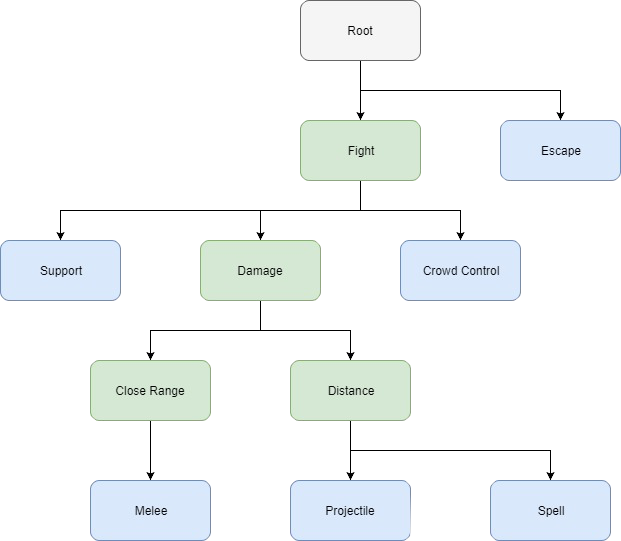
\includegraphics[scale=.35]{behavior_tree}}
	\caption{Behavior Tree}
	\label{fig: Behavior Tree}
\end{figure}
Figure \ref{fig: Behavior Tree} highlights the flow of decisions the A.I. will make before arriving
at an action. In this tree, each node represents a calculation that will affect the
branch that is taken, and each leaf represent an action.
\begin{figure}[H]
	\centering
	\centerline{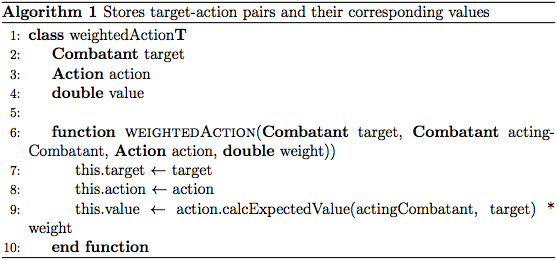
\includegraphics[scale=.37]{algorithm_1}}
	\caption{Algorithm 1}
	\label{fig: Algorithm 1}
\end{figure}
Algorithm 1 details the \textit{weightedAction} class. This class is used to store the
target-action pairs for a given combatant. It takes as input a target, acting combatant,
action and weight. \textit{actingCombatant} is the combatant that is currently
making the described action. \textit{target} is a \textit{Combatant} object within range of the acting combatant. \textit{action} is the specific attack or spell being used on the target.
\textit{value} is the overall measure of the effective of the action being performed on the
target by the acting combatant.

\begin{figure}[H]
	\centering
	\centerline{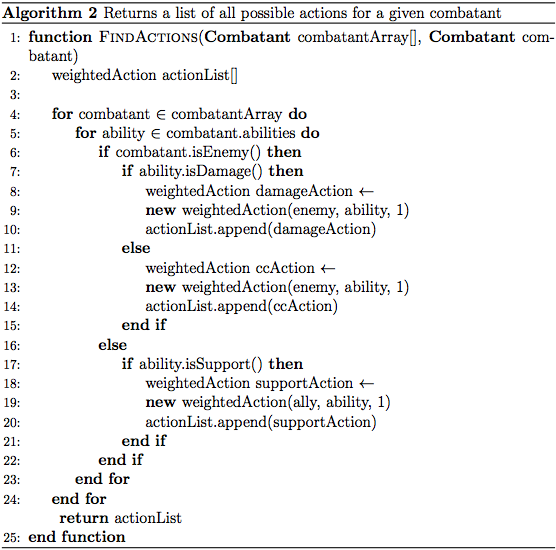
\includegraphics[scale=.37]{algorithm_2}}
	\caption{Algorithm 2}
	\label{fig: Algorithm 2}
\end{figure}
Algorithm 2 begins by iterating over the list of all combatants in the encounter.
For each enemy combatant in the encounter, we iterate over all abilities available
to our active combatant. We then check which category the selected ability is
a part of. For each category of ability, we create a new \textit{weightedAction} class,
passing in the ability and the target of that ability. Additionally, we pass in a
weight value. For this pseudocode, we assign the weight of each type of action to
be equal. In practice, the weight of each action would be adjusted to tweak the
behavior of each individual unit.

\begin{figure}[H]
	\centering
	\centerline{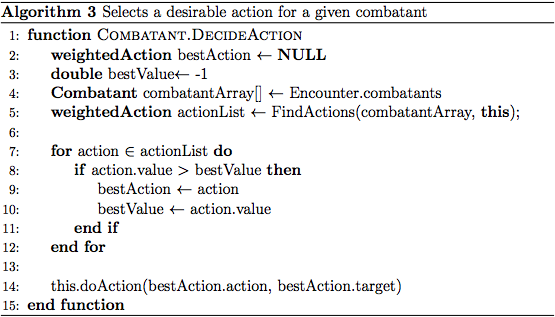
\includegraphics[scale=.37]{algorithm_3}}
	\caption{Algorithm 3}
	\label{fig: Algorithm 3}
\end{figure}
Algorithm 3 is the primary method used by a combatant to select an action.
The method iterates over the action list received from \textit{FindActions()}, and extracts
the one with the highest value. Once the action with the highest value has
been determined, we execute that action with \textit{this.doAction()}.

\begin{figure}[H]
	\centering
	\centerline{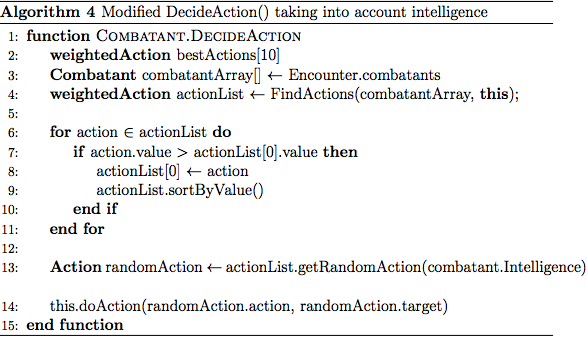
\includegraphics[scale=.37]{algorithm_4}}
	\caption{Algorithm 4}
	\label{fig: Algorithm 4}
\end{figure}

We developed an algorithm for better choosing an action for an A.I. combatant to take, detailed in Algorithm 4 (Figure \ref{fig: Algorithm 4}). It shows a modified\textit{ DecideAction()} method that selects a random
action from the top 10 most viable candidates based on the combatant’s intelligence
rating. This is currently not supported in our A.I. algorithm but we felt it was important to note that it is possible in the future of Critical Encounters.

\subsubsection{Encounter Diagnostic Tool}
The Encounter Diagnostic Tool, or EDT, will be a feature available to
users of the website to evaluate their encounter designs and receive highly detailed
evaluation based on a variety of metrics. Because combat in the d20 Game System
is quite extensive and highly open ended, it is unlikely that a user seeking to
create a well balanced and fluid encounter will be able to do so with some trial
and error. Instead of manually playing the encounter repeatedly with multiple
variations to check for weaknesses in the design, users will be able to run the
built in EDT to automatically generate useful information
regarding their encounter.
\begin{itemize}
	\item \textit{Interface:} The user will be able to access the interface for the EDT
	from within the encounter page, accessing the different parameters in the sidebar.
	The EDT option will only be available on encounters that
	the user has created, which is why we placed it in the encounter creator itself.
	Once the user has entered the parameters to run the EDT, they
	will be prompted to enter details necessary to configure the tests. \\
	\item \textit{Diagnostics Measurement:} When activated, the EDT will generate a set of valid party
	member compositions that meet both the restrictions of the encounter as well as
	the additional restrictions provided by the user during configuration. A party
	composition is a collection of player characters that will be placed on the field of
	play at the start of the encounter. The EDT will generate one party
	composition per iteration of the test. Once all party compositions are generated,
	the diagnostic tool will simulate the encounter one time for each party composition.
	The simulation will consist of each member of the party being placed in the
	user designated spawn positions for the encounter. Once all player characters
	are placed, both PC and GM turns will be taken by the A.I. until either side
	meets their win condition, at which point the board is reset and the next party
	composition is tested. Once all party compositions have been tested, the diagnostic
	tool serves the results of the tests to the user. It is not possible for the user to provide any input once the EDT has started, and an animation will play as the testing occurs to provide the user proof that the EDT is progressing. During each test, statistics relating to the performance of each entity in the
	encounter will be tracked in order to provide metrics by which the user can evaluate
	their encounter. Statistics that will be tracked include the following: Number of kills/deaths for each non-PC entity, number of kills/deaths by each PC entity, overall win rate of PC vs. GM, most damage given/taken, turn count, and a heat map to visualize where the most action has taken place. \\
	\item \textit{Results and Presentation:} One all simulations are complete and the data has been collected, it must be
	processed into a form that is quick and easy to understand. Each statistics that
	was tracked on a per-encounter basis will be aggregated into an average value and
	presented to the user in a separate window. These average values will highlight
	at a glance measurements such as the average length of each encounter, which
	enemies are the most dangerous, how difficult the overall encounter is, and which
	abilities are the most effective in the encounter. Additionally, a heat map will be
	generated using the location of kills made on the map across all simulations. This
	heat map will indicated to the user the general flow of combat, which can be used
	to help fine tune the encounter and improve overall quality.
\end{itemize}
After an encounter has been perfected by the user using the Battlefield in
Creation Mode users have the option to post it into their public Arena page for
other users’ to experience. Once it has been published to an Arena, the encounter
may be accessed via the Encounter Browser. The browser functions as a search bar
that allows users to find encounters made by other members of Critical Encounters.
Encounters can be located by matching the keywords the user searches with the
keywords associated with the encounter. These keywords can include the name
of the encounter, the type of encounter, location, level range, party size, difficulty
level, etc.

\section{Conclusions}

Tabletop games bring people together in a world where physical interaction is
often lost in lieu of digital communication. This project aims to supplement these
interactions by making them more accessible to newer players, as well as help
experienced players spend less time on pre-game preparation. In-game encounters
require large amounts of time to plan, setup, and implement, so by enhancing
this process and giving the GM the ability to perfect an encounter beforehand the
whole process becomes more enjoyable for anyone playing the game.
\par Critical Encounters has the potential to broaden the audience of an already quickly
expanding pastime to younger players and DM’s. Concepts in the realm of tabletop
games are very easily understood by a younger audience, as their imagination and
creativity can run free in such games. However, the threshold of understanding
for the many rules and balances may prove a bit overzealous for this audience.
Having a service that improves accessibility to newer players  also bleeds
into improving accessibility for younger players as well. Additionally, users who
do not have a group to play with may find and form groups with other users with
whom they have played and shared content with.

\section*{APPENDIX}

\listoffigures

\begin{thebibliography}{99}

\bibitem{c1} T. Coleman 2016. 'Meteor API Docs'. http://docs.meteor.com/.
\bibitem{c2} 'MongoDB Documentation'. https://docs.mongodb.com/. 2017.
\bibitem{c3} Michel Weststrate 2017. 'MobX'. https://mobx.js.org/.
\bibitem{c4} Wizards of the Coast 2016. 'Systems Reference Document (SRD). http://dnd.wizards.com/articles/features/systems-reference-document-srd.
\bibitem{c5} B. Vaughn 2017. 'Hello World'. https://reactjs.org/docs/hello-world.html.

\end{thebibliography}




\end{document}
